Before we started coding we made a draft of the class diagrams. Throughout the following sprints we kept maintaining and updating the class diagram
draft to make sure that the code and class diagram were in agreement. The class diagram shown and explained below is the final version for our
system.

The class diagram is the main building block of object oriented modelling. It is used both for general conceptual modelling of the systematics 
of an application and for modelling translating models into programming code. Class diagrams can also be used for data modeling. The classes in a 
class diagram represents both the main objects, interactions in the application and the classes to be programmed.

The class diagram is made in the Unified Modeling Language (UML) to ensure common understanding, when describing the structure of our system.

Overall the following class diagrams have been of great help throughout the programming of this application.

\begin{figure}[htb]
    \begin{center}
        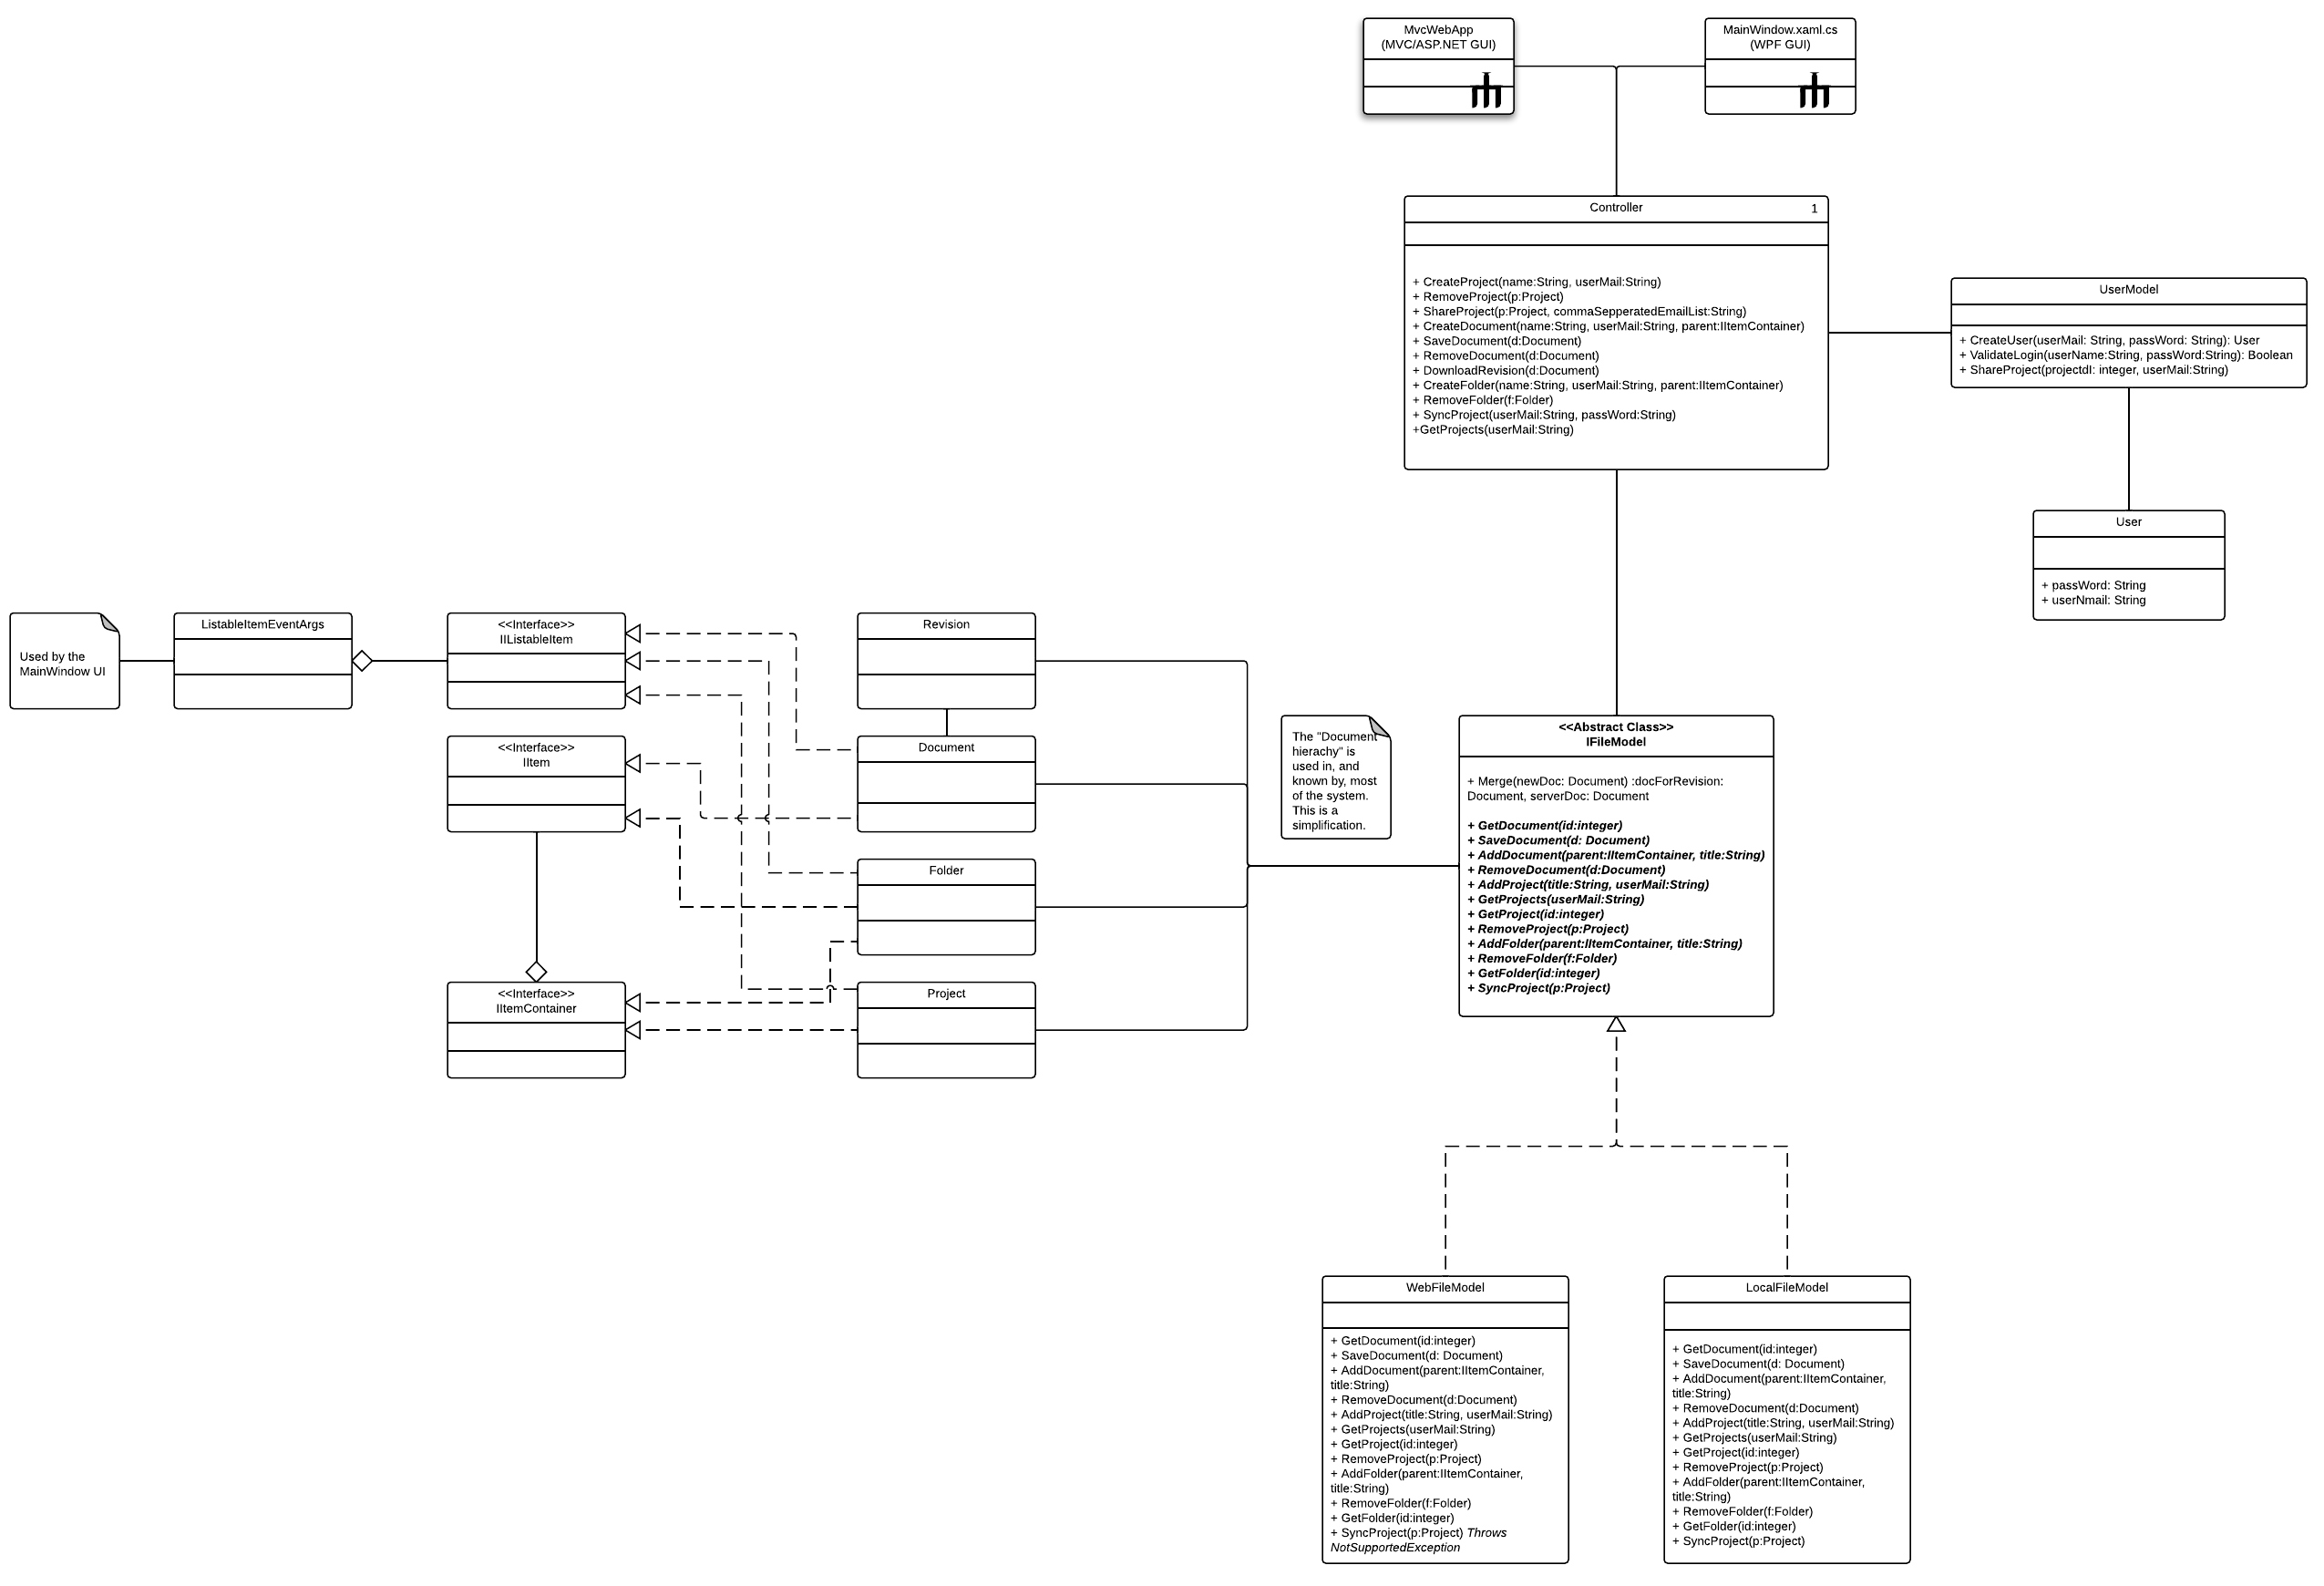
\includegraphics[width=1\textwidth]{Software_design/graphics/mainClassDiagram.png}
        \caption{Overview of the simplified main class diagram for 'Slice of Pie'}
        \label{fig:design-class_diagram} 
    \end{center}
\end{figure}

Due to its huge size we are not able to justify the illustration of this design class diagram in the report. For a zoomable version of the diagram, please go to 
\url{https://www.lucidchart.com/publicSegments/view/50b23e81-d30c-41d6-b6d1-3b9d0ac63d8b/image.png}.

In (Figure~\ref{fig:design-class_diagram}) the most critical and important classes are shown with their most important attributes and public methods.
None of the two GUIs (MvcWebApp and MainWindow) are shown in the class diagram, but are in two separate class diagrams. This is shown with the rake
symbol on the two classes in the main class diagram.

As the class diagram shows, we have made one controller that is responsible for all the method calls between the views and back end models. We have an abstract
IFileModel class, from which both the WebFileModel and LocalFileModel inherits. Left to the abstract IFileModel class, we have made a simplification of the folders and 
documents hierachy. 

Furthermore do we also have a UserModel that takes care of the way users interact with the FileModels. The UserModel also takes care of creating users. All that is needed
to create a user is an email address and a password. Even though a user tries to sign in, but does not exist in the database a user is created.

\subsubsection{The MvcWebApp GUI}

The diagram showing the raked class diagram for the MvcWebApp GUI can be found in the Appendix~\ref{fig:mvcwebapp-diagram}.

We have chosen only to show the controller classes, since they are the most crucial classes for understanding how the Web UI works. The Web UI uses
the ASP.NET MVC3 Framework. We decided to use MVC since we thought it to be suitable for our needs.

The 'views' of the MVC3 structure has been omitted. This is done because they do not have any important or interesting functionality except of rendering
the different sites that are available at the Web UI. The methods with a [GET] tag, gets a desired view and the methods with a [POST] tag, posts a HTTP request.

For each method in a controller there is a corresponding view that is rendered when the method is called. However if there are two methods with the same 
name in a controller, where one is a [GET] method and the other is a [POST] method, there is only one view.

The 'models' used are all located in the 'SliceOfPie' project which ensures that consistency between the Web client and the local client.


The ASP.NET MVC3 Framework ensures a very clear separation between the models, views and controllers (MVC design pattern) of the web application. It makes a web application 
very scalable and easy to maintain or expand. Another great side of the ASP.NET MVC3 Framework is the use of HTML5.

\subsubsection{The MainWindow GUI}

The diagram showing the raked class diagram for the MainWindow GUI is to be found in the Appendix~\ref{fig:mainwindow-diagram}.

As well as with the raked MvcWebApp GUI class diagram we have chosen only to show the most crucial classes and methods in this raked diagram. We have used WPF for
the GUI for the local client. All GUI code is written in .xaml.cs files with some helper methods.
% Talk to Niclas about what else there is to say about this.

